The high-luminosity upgrade for the LHC planned to be ready to run in 2026 imposes new challenges on detectors. For instance, an enhanced luminosity is immediately related to elevated radiation levels which constitute heat development. To avoid a thermal runaway and ensure reliable measurements, the electronics must be held at a constant temperature\todo{How cold should it be?}\ which requires some kind of cooling system for all detector components.

\subsection{Petal}
The summer student project documented in this report was related to the thermal performance tests of the inner tracking detector of the ATLAS experiment. Figure \ref{fig:ATLAS} illustrates its position within the big detector and the planned upgraded design. The parts studied at DESY are the so-called petals that are assembled perpendicularly around the beampipe to track particles with low transversal energy. Figure \ref{fig:petal} displays a picture of the tested petal prototype.
\begin{figure}[h!]
	\centering
	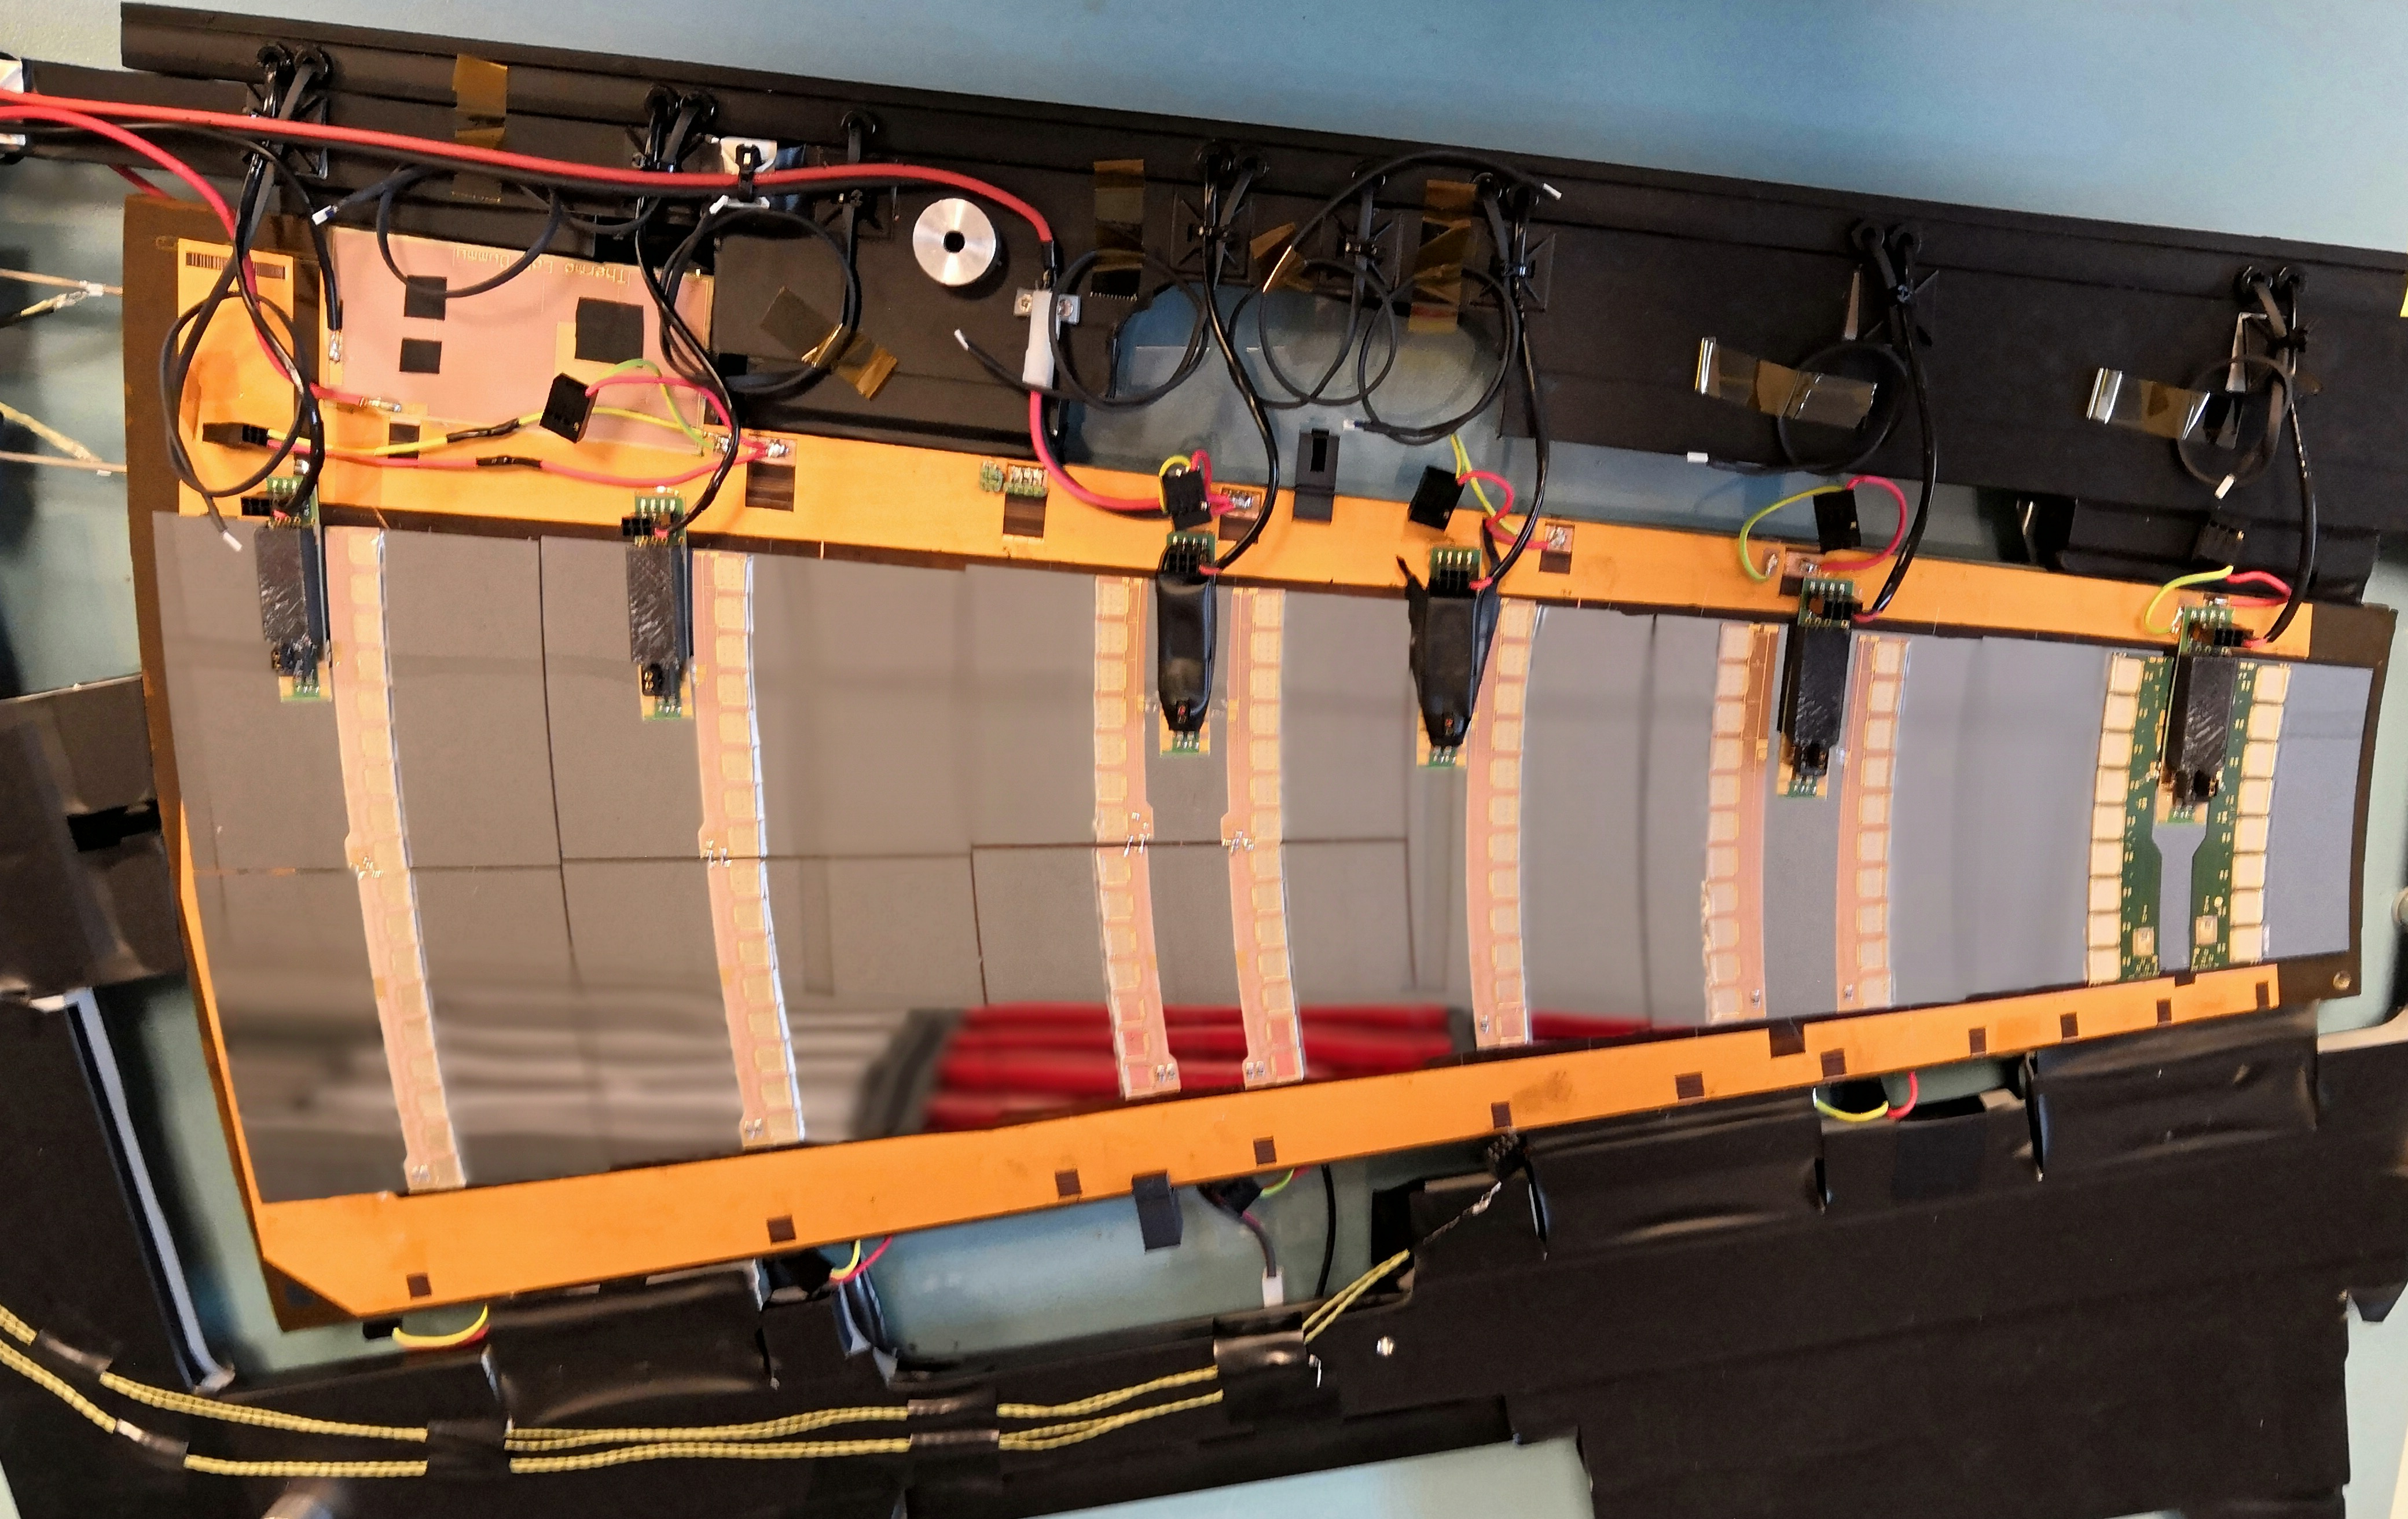
\includegraphics[width=.6\textwidth]{img/petal.jpg}
	\caption{Picture of the tested petal prototype.}
	\label{fig:petal}
\end{figure}
\subsection{Cooling System}
Figure \ref{fig:coolingLoop} shows a prototype of the bare cooling loop. The cooling system is based on the energy needed for a phase change. Liquid $\text{CO}_2$ is pumped into the cooling loop where some of it evaporates if exposed to heat. This evaporation requires energy (enthalpy of evaporation) which is taken from the heat source.
\begin{figure}[h!]
	\centering
	\tikz[baseline=(a.north)]\node[yscale=-1,inner sep=0,outer sep=0](a){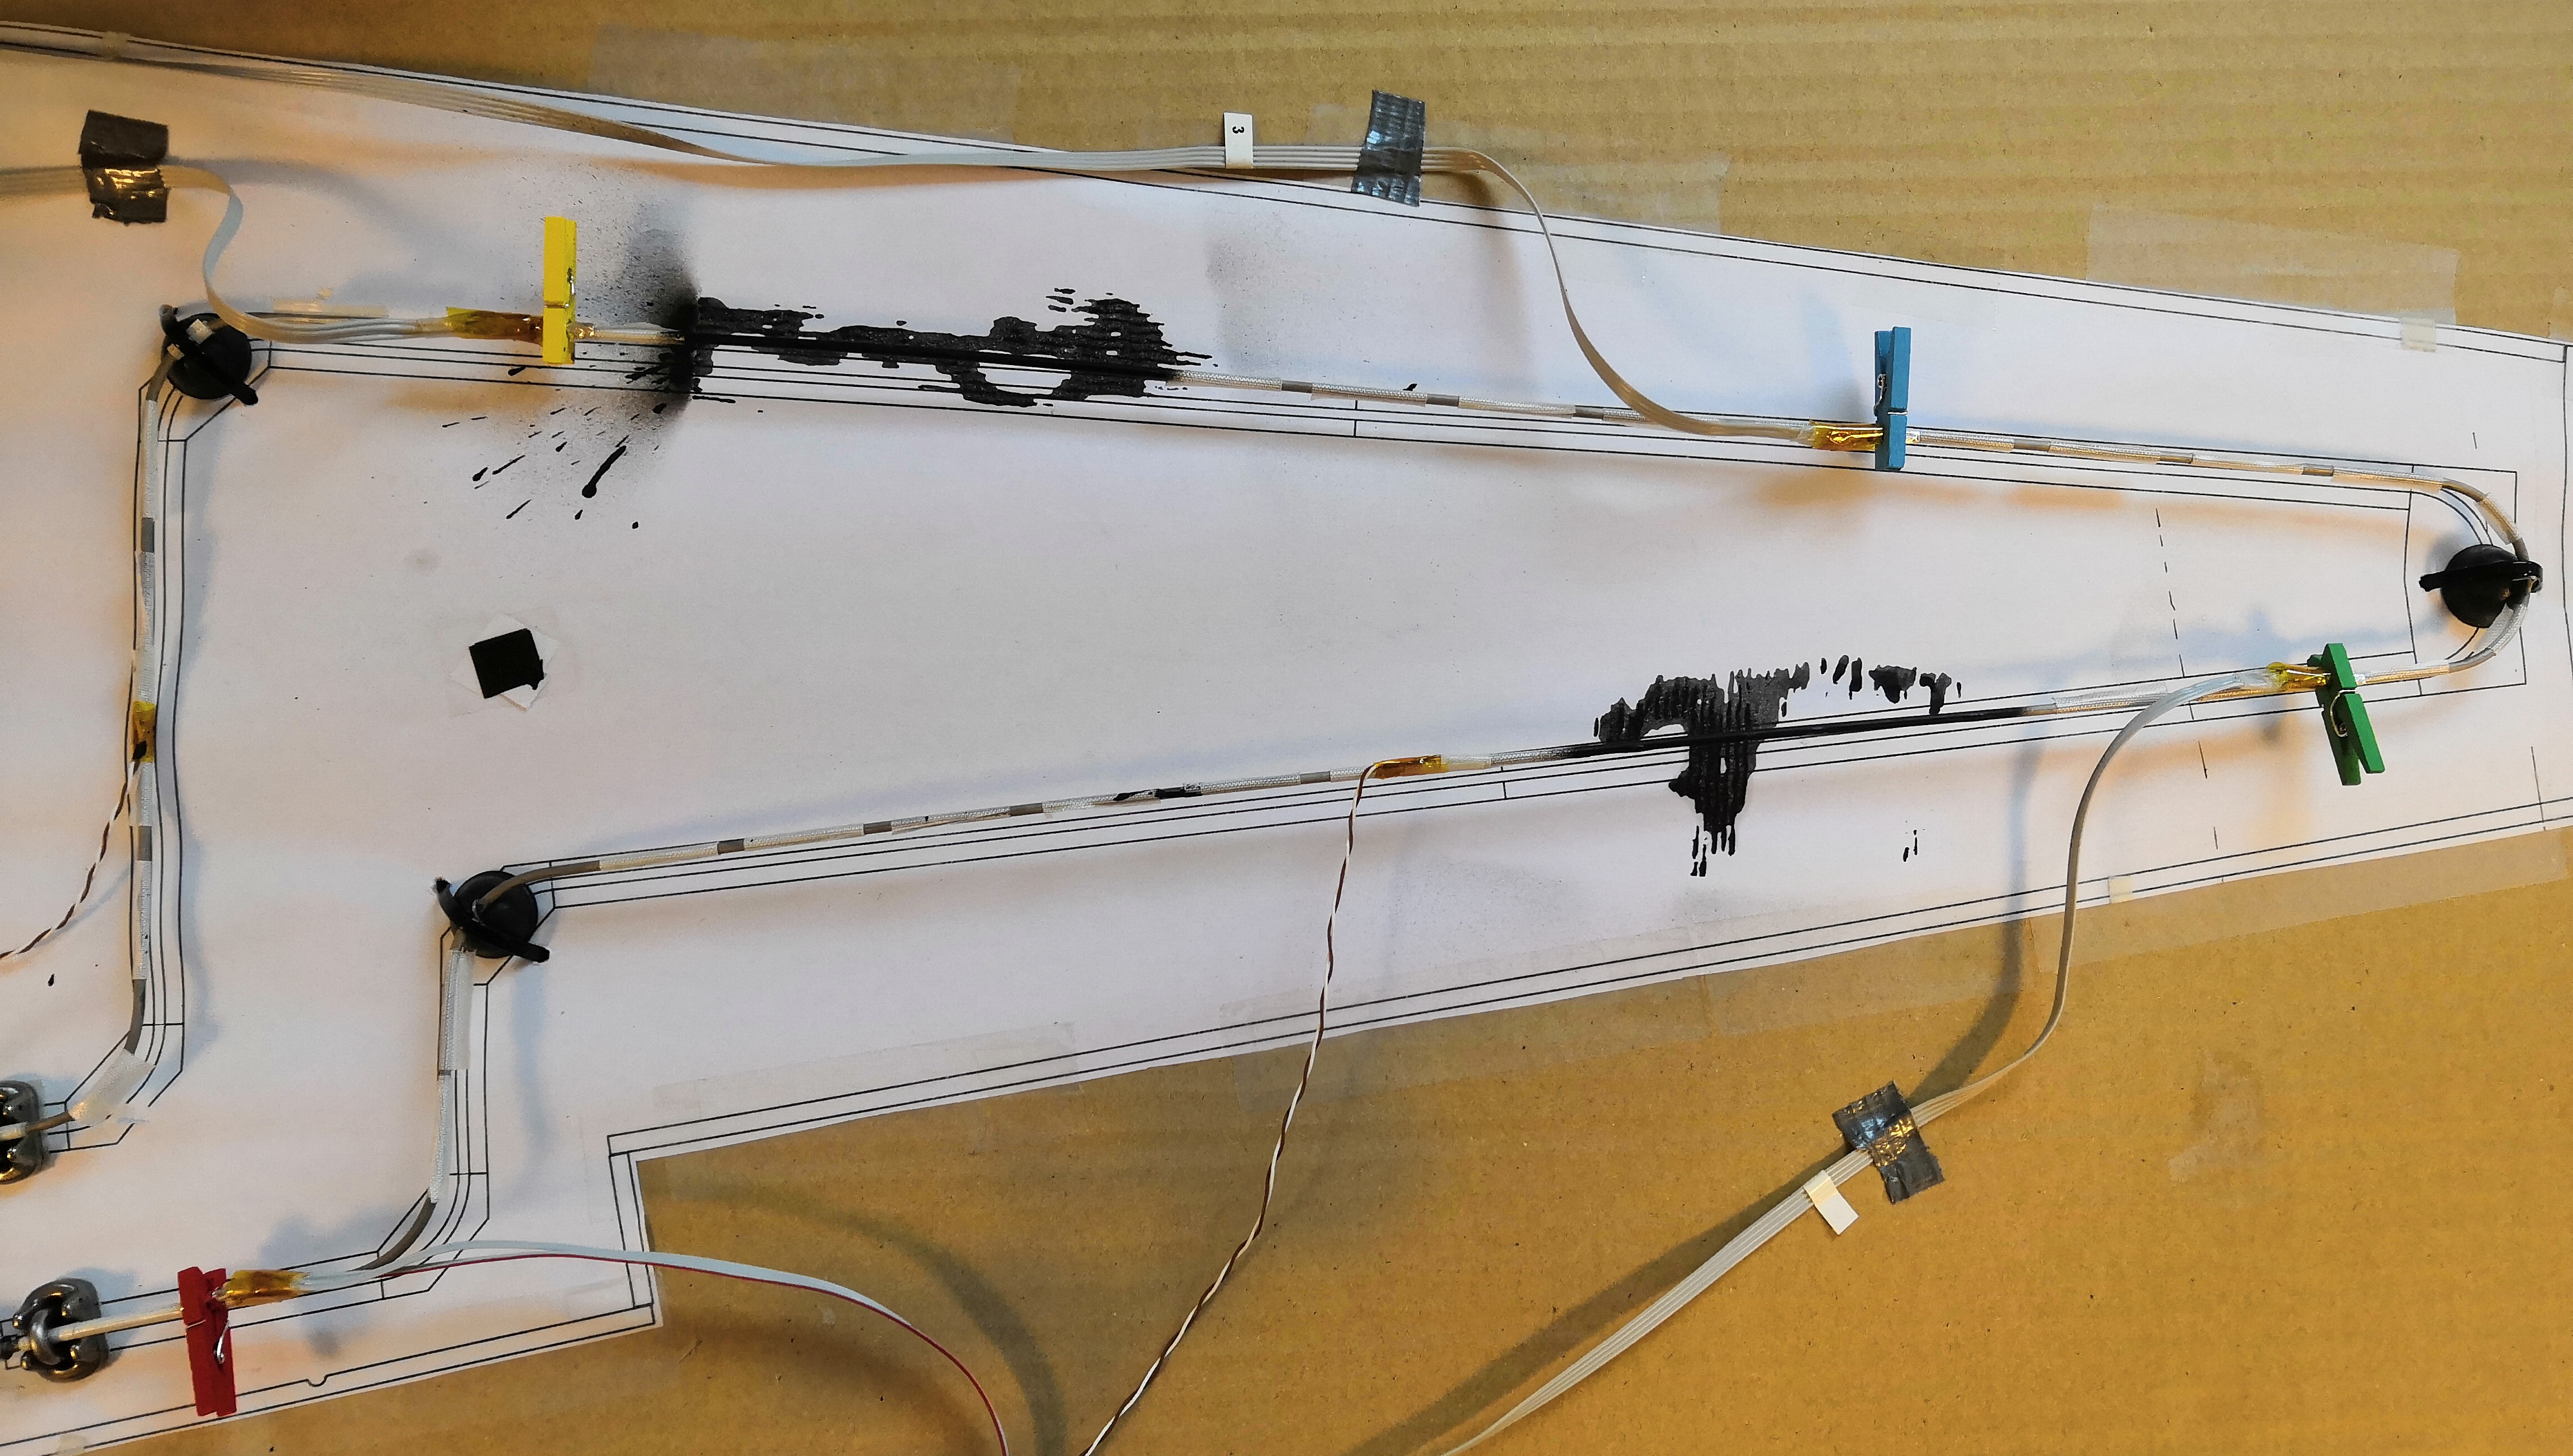
\includegraphics[width=.6\textwidth]{img/coolingLoop.jpg}};
	\caption{Picture of the a bare cooling loop.}
	\label{fig:coolingLoop}
\end{figure}

\begin{landscape}
\begin{figure}[h!]
	\centering
	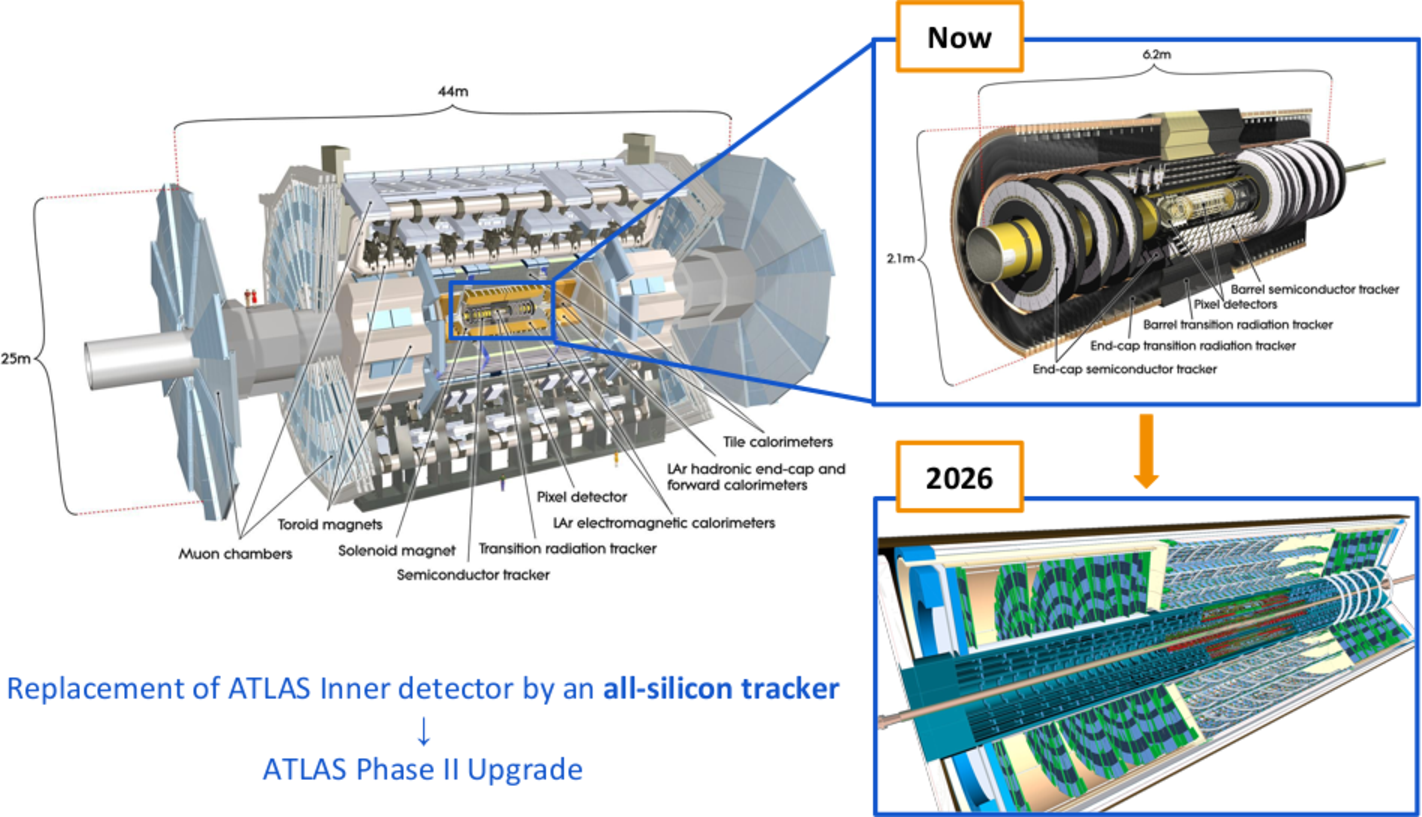
\includegraphics[height=0.9\textwidth]{img/ATLAS.pdf}
	\caption{Schematics of the upgrade of the ATLAS inner tracking detector.}
	\label{fig:ATLAS}
\end{figure}
\end{landscape}